\documentclass[a4paper,conference]{IEEEtran}

\usepackage[utf8]{inputenc}
\usepackage{amsfonts}
\usepackage{amssymb}
\usepackage{graphicx}
\usepackage{array}
\usepackage[cmex10]{amsmath}
\usepackage{multirow}
\usepackage{algorithmic}

\begin{document}

\title{Exploration of energy efficient memory organisations for dynamic multimedia applications using scenarios}
\author{\IEEEauthorblockN{Iason Filippopoulos\IEEEauthorrefmark{1},
Francky Catthoor\IEEEauthorrefmark{2} and
Per Gunnar Kjeldsberg\IEEEauthorrefmark{1}}
\IEEEauthorblockA{\IEEEauthorrefmark{1}Department of Electronics and Telecommunications\\
Norwegian University of Science and Technology,
Trondheim, Norway\\ Email: iason.filippopoulos@iet.ntnu.no}
\IEEEauthorblockA{\IEEEauthorrefmark{2}IMEC, Kapeldreef 75, 3000 Leuven, Belgium\\}}

\maketitle

%Re-written by PGK
\begin{abstract}
We propose a memory-aware system scenario approach that exploits variations in memory needs during the lifetime of an application to optimize energy usage. Different scenarios capture the application’s different resource requirements which change dynamically at runtime. In addition to computational resources, the many possible memory platform configurations and data-to-memory mappings are among the most important scenario parameters. Here we present an extended memory model that includes existing state-of-the-art memories, available in the industry and academia, and show how it is employed during the system design exploration phase. Both commercial SRAM and standard cell based memory models are explored in this study. The effectiveness of the proposed methodology is demonstrated and tested using a large set of multimedia benchmarks published in the Polybench, Mibench and Mediabench suites. Reduction in energy consumption in the memory subsystem of up to 55 \% is shown.
\end{abstract}
\IEEEpeerreviewmaketitle

\section{Introduction}
\label{sec:introduction}
\footnotetext{Version 04.04.2013: Third iteration of comments and PGK's abstract}

Modern embedded systems are becoming more and more powerful as the semiconductor processing technique keeps increasing the number of transistors on a single chip. Consequentially, demanding applications, such as signal processing and multimedia applications, can be executed on these devices \cite{narasinga}. On the other hand, the desired performance has to be delivered with the minimum power consumption due to the limited amount of power offered in mobile devices \cite{tcm}. System scenario methodologies propose the use of different platform configurations in order to exploit variations in computational and memory needs often seen during the lifetime of such applications \cite{tcm}. 

%Francky: explain about the knobs
With regard to the memory-aware system scenario methodology, a platform can be reconfigured through a number of potential knobs and each knob consequentially results to different performance and power consumption on memory subsystem. Foremost different energy states are supported on modern memories through power gating techniques and certain memory units could be switched on lower power modes when not accessed \cite{Fil12}. The second platform knob is the mapping of data to the available memory banks. The data mapping decisions affect both the energy per access for the mapped data, the data conflicts as a result of suboptimal mapping and the number of active banks. In this work a reconfigurable memory platform is constructed using detailed memory models and some dynamic multimedia applications are employed in order to study the effectiveness of the methodology.

%Domain specific for ESTIMedia + comparison with use case
The main contribution of the current work in comparison with \cite{Fil12} is the usage of more accurate and detailed memory models on the system design exploration, the extended number of benchmark applications on which the methodology is applied and the categorisation of applications, based on their dynamic characteristics. Especially with regard to the multimedia domain, the current work presents a comprehensive methodology for optimising energy consumption on memory subsystem, which is potentially applicable to every multimedia application with dynamic memory usage. In addition, in this study the scenarios are based on the actual behaviour of the system in contrast to use case scenario approaches in which scenarios are generated based on user's behaviour.

This paper is organized as follows. Section~\ref{sec:motivation} discusses the motivation for the study of optimizations on memory organisation. Section~\ref{sec:related} surveys related work on system level memory exploration and on system scenario methodologies. The main contribution of the current study in comparison with that work is also presented in section~\ref{sec:related}. Section~\ref{sec:methodology} presents the chosen methodology with main focus on the memory organisation study. In Section~\ref{sec:platform} the target platform is described accompanied a detailed description of the employed memory models, while the multimedia benchmarks and their characteristics are analysed in Section~\ref{sec:applications}. Results of applying the described methodology to the targeted applications are shown in Section~\ref{sec:results}, while conclusions are drawn in Section~\ref{sec:conclusion}. 

\section{Motivation}
\label{sec:motivation}

As shown in \cite{Gonzalez1996} memory contributes around 40\% to the overall power consumption in general purpose systems. Especially for embedded systems, the memory subsystem accounts for up to 50\% of the overall energy consumption \cite{Che09} and the cycle-accurate simulator presented in \cite{Ben99} estimates that the energy expenditures in the memory subsystem range from 35\% up to 65\% for different architectures. The breakdown of power consumption for a recently implemented embedded system presented in \cite{Hul11} shows that memory subsystem consumes more than 40\% of the leakage power on the platform. According to \cite{tcm}, conventional allocation and mapping of data done by regular compilers is suboptimal. Performance loss is caused by stalls for fetching data and data conflicts for different tasks, due to the limited size of memory and the competition between tasks. 

In addition, modern applications exhibit more and more dynamism. This dynamism is reflected also on memory resources and techniques have developed in order to estimate the storage size requirements of applications in a systematic way \cite{Ang13}. The significant contribution that the memory subsystem has in the overall energy consumption of a system and the dynamic nature of many applications offer a strong motivation for the study and optimization of memory organisation in modern embedded devices.

%F: motivation example added
To illustrate the aforementioned sub-optimal conventional allocation and mapping of data, the simple example in Fig.~\ref{fig:motivation} is used. The kernel code of an image processing application continuously read images and performs a \textit{foo} function on each pixel of the image. Normally an array is used for saving the intermediate calculations in image processing applications, which is declared as \textit{array} in the motivation example. The memory size used for storage of \textit{array}  is defined by the dimensions of the \textit{image} and can be potentially different for a series of input images. In a conventional mapping the highest values of \textit{height} and \textit{width} are identified and a static compiling results in allocation of the worst-case area for \textit{array}. However, only a part of the allocated space is accessed during processing of smaller images. The proposed methodology tries to optimise the memory usage for dynamic cases similar to the simplified motivation example.

\begin{figure}[!t]
\begin{algorithmic}
\WHILE{$image \ne 0$}
	\STATE $height \gets length(image)$
	\STATE $width \gets width(image)$
	\FOR{$i = 0 \to height$} 
		\FOR{$j = 0 \to width$} 
			\STATE $array[i][j] \gets foo(image[i][j])$
		\ENDFOR
	\ENDFOR
\ENDWHILE
\end{algorithmic}
\caption{Motivation example of dynamic memory usage}
\label{fig:motivation}
\end{figure}

\section{Related Work and Contribution Discussion}
\label{sec:related}
%PGK: Try to find newer examples

Many papers have focused on memory related optimisations, also in the presence of a partitioned and distributed memory organisation with memory blocks of different sizes. In \cite{Ben00b} authors present a methodology for automatic memory hierarchy generation that exploits memory access locality, while in \cite{Ben00c} they propose an algorithm for the automatic partitioning of on-chip SRAM in multiple banks that can be independently accessed. Several design techniques for designing energy efficient memory architectures for embedded systems are presented in \cite{Mac02}. In \cite{Pgk01} data and memory optimization techniques, that could be dependent or independent of a target platform, are discussed . 

Energy-aware assignment of data to memory banks for several task-sets based on MediaBench is presented in \cite{Mar03}. Low energy multimedia applications are discussed also in \cite{Chu02} with focus on processing rather than memory platform. However, both the aforementioned works perform their analysis based on use case situations and do not incorporate sufficient support for very dynamically behaving application codes. System scenarios allow to alleviate this bottleneck and to handle such dynamic behaviour. In addition, the current work explores the mapping of data to the memory and the effect of different mapping decisions on the overall energy consumption.

An overview of work on system scenario methodologies and their application are presented in \cite{Gheorghita2007}. In \cite{Fil12} the extensions towards a memory-aware system scenario methodology are presented and demonstrated using theoretical memory models and two target applications. This work is an extension both in complexity and accuracy of the considered memory library and on the number of target applications. 

Furthermore, the majority of the published work focus on control variables for scenario prediction and selection. Control variables can take a relatively small set of different values and thus can be fully explored. However, the use of data variables \cite{Elena2010} is required by many dynamic systems including the majority of multimedia applications. The wide range of possibly values for data variables is higher and makes full exploration impossible. Most of the dynamic variables in the current work can be classified as data variables due to their significant variation under different execution situations. 

Authors in \cite{Pal06} present a technique to optimise memory accesses for input data dependent applications by duplicating and optimising the code for different execution paths of a control flow graph (CFG). One path or a group of paths in a CFG form a scenario and its memory accesses are optimized using global loop transformations (GLT). Apart from if-statement evaluations that define different execution paths, they extend their technique to include while loops with variable trip count in \cite{Pal06b}. A heuristic to perform efficient grouping of execution paths for scenario creation is analysed in \cite{Pal07}. However, our work extends the existing solutions towards exploiting the presence of a distributed memory organisation with reconfiguration possibilities.

Reconfigurable hardware for embedded systems, including the memory architecture, is a topic of active research. An extensive overview of current approaches is found in \cite{Garcia}. The approach presented in this paper differentiates by focusing on the data-to-memory partitioning aspects in the presence of a platform with dynamically configurable memory blocks. 

\section{Memory-Aware System Scenario Methodology}
\label{sec:methodology}
%PKG: Remove most of the citations to Norchip

The memory-aware system scenario methodology is based on the observation that the workload on memory subsystem varies significantly on time due to dynamic variation of memory needs in the application code. Most of the existing design methods define the memory requirements of the most demanding task and tune the system in order to meet its needs \cite{tcm}. Obviously, this approach leads to wasted memory area for tasks with lower memory requirements, since those tasks could meet their needs using fewer resources and consequentially consuming less energy. Another source of unnecessary waste of energy on the memory is the data conflicts due to misplaced data. Replacement of old data and fetching of new data is both time and energy consuming and should therefore be avoided. Handling of data conflicts is also part of the  memory-aware system scenario methodology.

In contrast, designing with scenarios is workload adaptive and offers different configurations of the platform and the freedom of switching to the most efficient scenario at run-time. In contrast to use case scenario approaches in which scenarios are generated based on a user's behaviour, the system scenario methodology focuses on behaviour of the system to generate scenarios. A system scenario is a configuration of the system that combines similar run-time situations (RTSs). An RTS consists of a running instance of a task and its corresponding cost (e.g. energy consumption) and one complete run of the application on the target platform represents a sequence of RTSs \cite{Elena2010}. The system is configured to meet the cost requirements of an RTS by choosing the appropriate scenario, which is the one that satisfies the requirements using minimal power.

In the following subsections, the different steps of the memory-aware system scenario methodology are outlined. A more detailed presentation of system scenario methodology and its extensions to make it applicable in a memory organisation study can be found in \cite{Fil12}.

\subsection{General Description of Memory-Aware System Scenario Methodology}

The scenario methodology follows a two stage exploration, namely design-time and run-time stages, as described in \cite{Gheorghita2007}, which is also employed in the memory-aware extension of the methodology. The two stage exploration is chosen because it reduces run-time overhead while preserving an important degree of freedom for run-time configuration \cite{tcm}. In more detail, the application is analysed at design-time and different execution paths causing variations in memory demands are identified. This procedure, which is time consuming and as a result can be performed only during the design phase, will result in a grey-box model representation of the application. The grey-box model hides all static and deterministic parts of the application, by providing only related memory costs for those, and keeps parts of the application code that are non-deterministic in terms of memory usage available to the system designer \cite{graybox}. 


\subsection{Design-time Profiling}

\begin{figure}[!t]
\centering
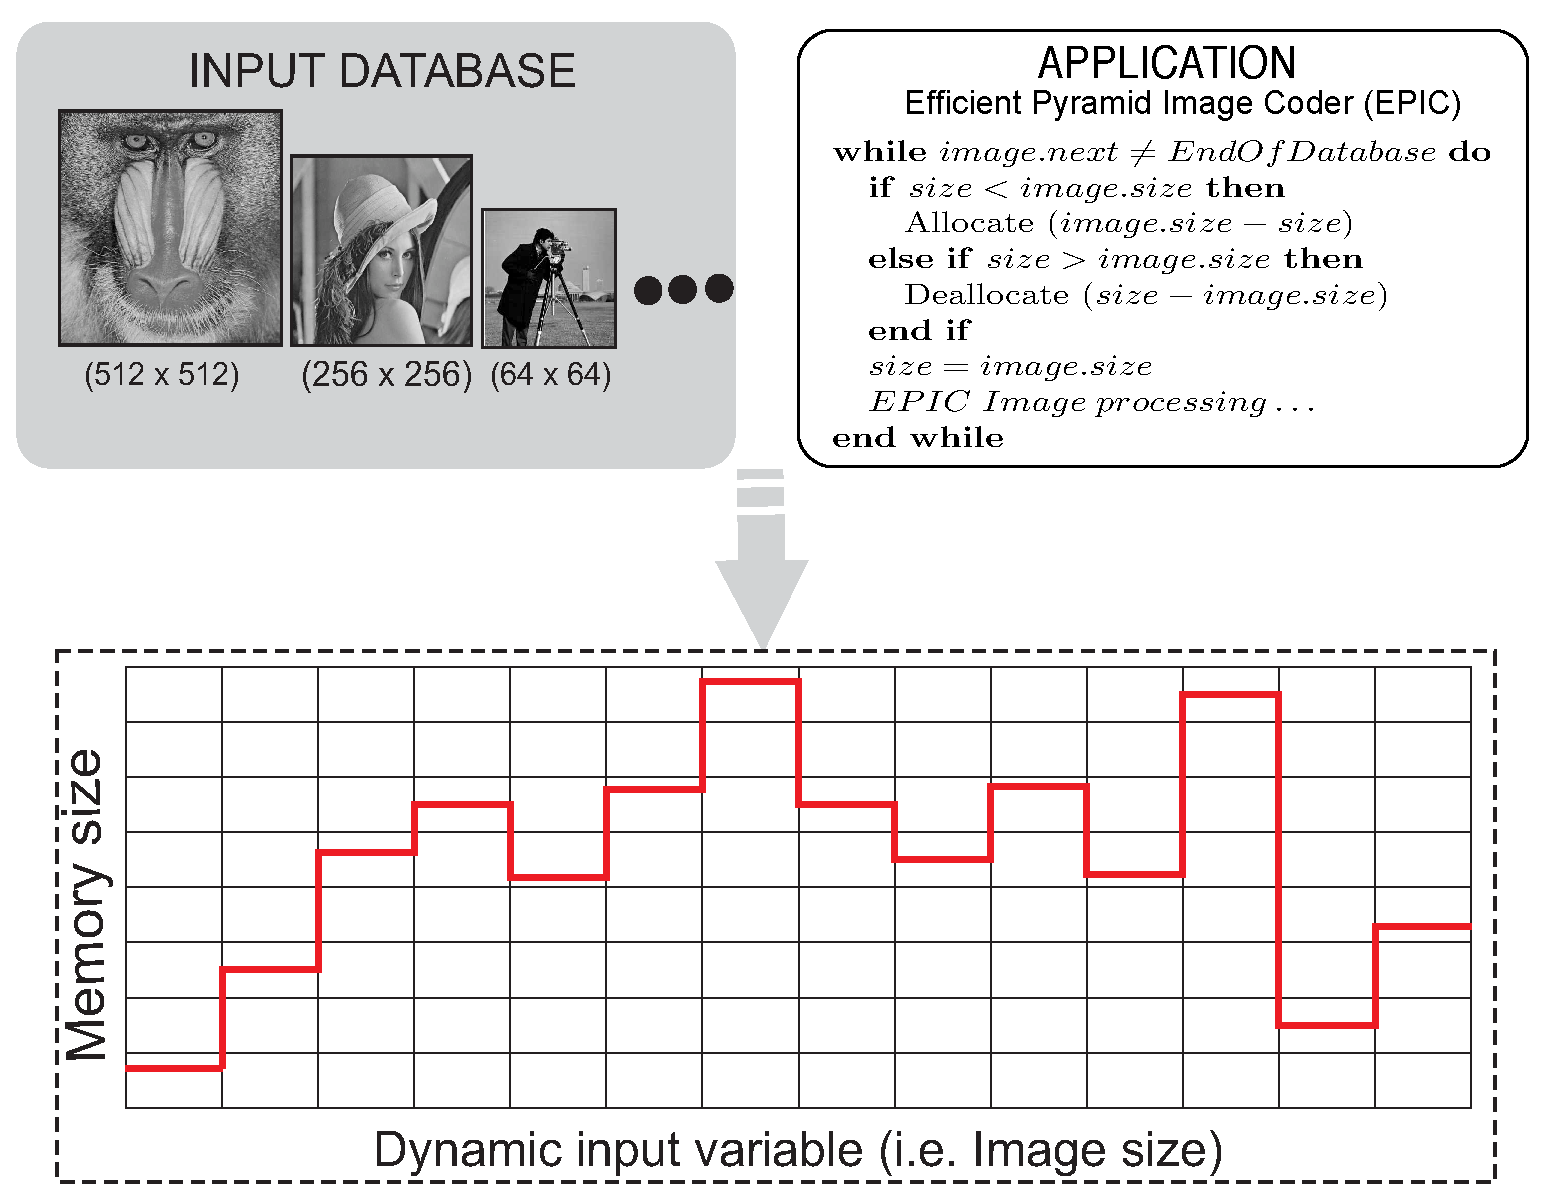
\includegraphics[width=0.45\textwidth]{Images/profiling2.eps}
\caption{Profiling results based on application code and input data.}
\label{fig:profiling}
\end{figure}

Application profiling is performed at design-time and consists of an analysis of the target application during its lifetime and for a wide range of inputs. The analysis focuses on the allocated memory size during execution and the variation in access pattern of the application. Techniques described in \cite{Ang13b} are used among others, in order to extract the access scheme. Several applications dynamically allocate and deallocate memory space during their execution, based both on the source code and the given input. 

The profiling stage is depicted in Fig.~\ref{fig:profiling} and consists of running the application code with suitable input data often found in a database, in order to produce profiling results. This reveals parts of the application code with high memory activity and with varying memory access intensity, which possibly depends on input data. Because of this behaviour, a static study of the application code alone is insufficient since the target applications for this methodology have non-deterministic behaviour that is driven by input. Choosing an extensive and accurate database is vital and will heavily influence and steer the designer's decisions in later steps. 

Given code and database as inputs, profiling will show memory usage during execution time by running the application using the whole database as an input. Results provided to the designer include complete information about allocated memory size values together with the number of occurrences and duration for each of these memory size values. Moreover, correlation between input data values and the resulting memory behaviour can possibly be observed. This information should be corporated to the clustering step that follows. 

In Fig.~\ref{fig:profiling} the profiled applications are two image related multimedia benchmarks and the input database should consist of a variety of images. The storage requirements in each case are driven by the current input image size. 

\subsection{Design-time Scenario Identification and Prediction}

\begin{figure}[!t]
\centering
\includegraphics[width=0.45\textwidth]{Images/1Dclustering.eps}
\caption{Clustering of profiling (a) results into three (b) or four (c) scenarios}
\label{fig:clustering}
\end{figure}

The next step is the clustering of profiled memory sizes into groups with similar characteristics, which is referred as scenario identification. Clustering is necessary, because it will be extremely costly to have a different scenario for every possible size, due to the amount of memories needed. Clustering neighbouring RTSs is a rational choice, because two instances with similar memory needs have similar energy consumption. 

In Fig.~\ref{fig:clustering} the clustering of the previously profiled information is presented. The clustering of RTSs is based both on their distance in memory size axis and the frequency of their occurrence. Consequentially, the memory size is split unevenly with more frequent RTSs having a shorter memory size range. In the case of a clustering to three scenarios the space is divided in the three differently coloured hashed areas depicted in Fig.~\ref{fig:clustering}(b). Due to the higher frequency of RTSs in the yellow hashed area that scenario is less wide compared to its neighbouring scenarios. That clustering is better compared to an even splitting of the area to three, because the energy cost of each scenario is defined by the upper size limit, as each scenario should support all RTSs within its range. Consequentially the overhead for the RTSs in the yellow area is lower compared to the overhead in the two other areas.

The same principal applies also when the number of scenarios is increased to five, as depicted in Fig.~\ref{fig:clustering}(c). The frequency sensitive clustering results in two short scenarios that contain four RTSs each and three wider scenarios with lower numbers of RTSs. The number of scenarios should be kept limited mainly due to two facts. First, implementation of a high number of scenarios in a memory platform is more difficult and complex. Second, the switching between the different scenarios involves an energy penalty that could become significant, when the switching takes place frequently.

The storage size and the frequency of each RTS are not the only two parameters that should be taken into consideration during the scenario identification. The storage size of each RTS results in a different energy cost depending on the way it is mapped into memory. The impact of the different mapping possibilities is included into clustering by introduction of the energy as a cost metric. The energy cost for each RTS is calculated using a reference platform with one to five memory banks. Increasing number of memory banks results in lower energy per access as the smaller and more energy efficient banks can be chosen for mapping of most frequently accessed elements and unused banks can be switched off.

A two dimensional space is used for clustering that also includes energy cost metric. For each RTS all different mapping options are studied. A Pareto curve that includes only the optimal mapping to the reference platform is constructed for each RTS. Suboptimal mappings that result in conflicts are not included in the Pareto curve. In Fig.~\ref{fig:pareto} four Pareto curves each corresponding to a different RTS are shown together with some energy cost levels corresponding to different data-to-memory mapping decisions. Pareto curves are clustered into three different scenarios based again both on their distance and frequency of occurrence. A smaller number of RTSs is depicted in Fig.~\ref{fig:pareto} compared to Fig.~\ref{fig:clustering}, although the numbering follows the clustering for the maximum number of scenarios. 

\begin{figure}[!t]
\centering
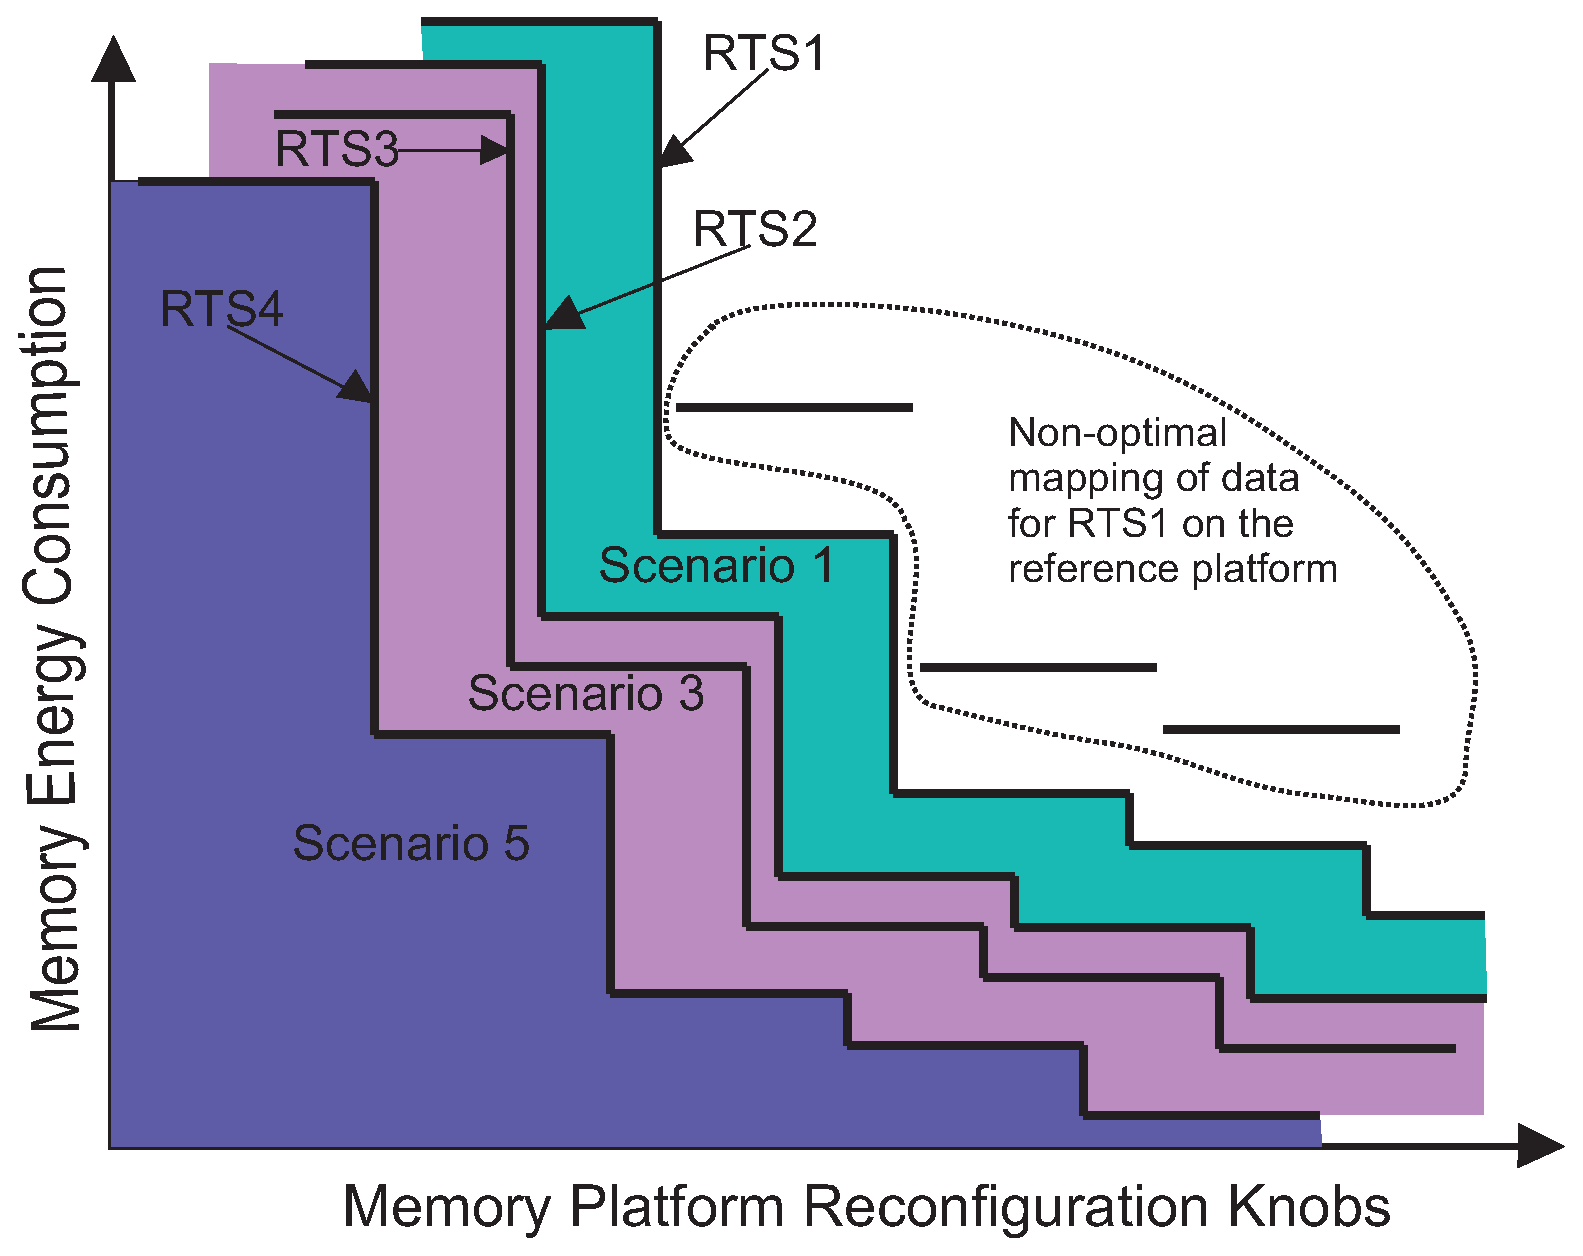
\includegraphics[width=0.45\textwidth]{Images/2DClustering.eps}
\caption{Clustering of Pareto curves}
\label{fig:pareto}
\end{figure}

The design-time scenario prediction phase consists of determination of the variables that define the active scenario. This can be achieved by careful study of the application code, combined with the application's data input. In our case the grey-box model reveals only the code parts that will influence memory usage, so that variables deciding memory space changes can be identified. An example of this is a non static variable that influences the number of iterations for a loop that performs one memory allocation at each iteration. In the depicted example the scenario prediction variable is the input image height and width values. Moreover, the designer should look for a correlation between input values and the corresponding cost. This information will be useful in the following steps of the methodology \cite{tcm}.

\subsection{Run-time}

Switching decisions will be taken at run-time by the run-time manager. The switching phase consists of all platform configuration decisions that can be made at run-time, e.g., frequency/voltage scaling, turning on/off a memory unit, and remapping of data on memory units. Switching takes place when the switching cost is lower than the energy gains achieved by switching. In more detail, the run-time manager compares the memory energy consumption of executing the next task in the current active scenario with the energy consumption of execution with the optimal scenario. If the difference is greater than the switching cost, then scenario switching is performed \cite{tcm}. Switching costs are defined by the platform and include all memory energy penalties for run-time reconfigurations of the platform, e.g., extra energy needed to change state of a memory unit.

\begin{figure}[!t]
\centering
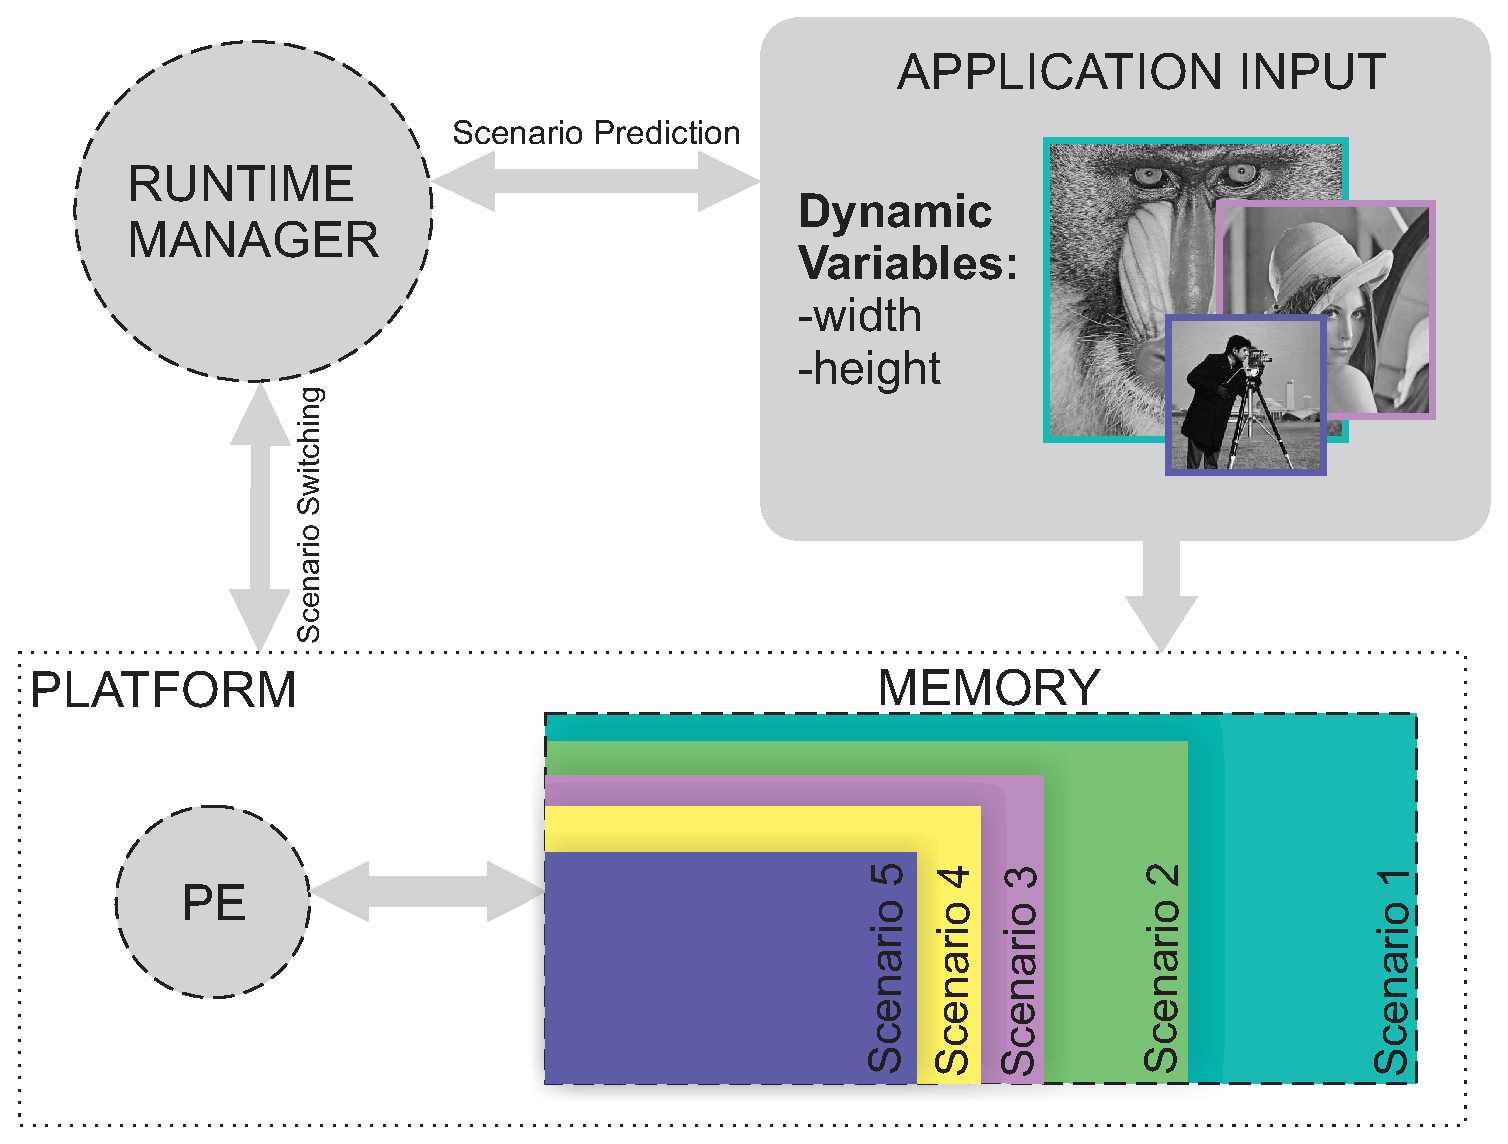
\includegraphics[width=0.45\textwidth]{Images/switching.eps}
\caption{Runtime scenario prediction and switching based on the current input}
\label{fig:runtime}
\end{figure}

In Fig.~\ref{fig:profiling} an example of the run-time phase of the methodology is depicted. Runtime manager identifies the size of the image that will be processed and reconfigures the memory subsystem on the platform, if needed, by increasing or decreasing the available storage size. The reconfiguration options are effected by platform hardware limitations.

\section{Target Platform}
\label{sec:platform}

Selection of target platform is an important aspect of the memory-aware system scenario methodology. The key feature needed in the platform architecture is the ability to efficiently support different memory sizes that correspond to the scenarios generated by the methodology. Execution of different scenarios then leads to different energy costs, as each configuration of the platform results in a specific memory energy consumption. The dynamic memory platform is achieved by organising the memory area in a varying number of banks that can be switched between different energy states. 

\subsection{Architecture}

In this work, a clustered memory organisations with up to five memory banks of varying sizes is explored. The limitation in the number of memory banks is necessary in order to keep the interconnection cost between the PE and the memories constant through exploration of different architectures. For more complex architectures the interconnection cost should be considered and analysed separately for accurate results. Although power gating can be also applied to the bus when only a part of a longer bus is needed, an accurate model of the memory wrapper and interconnection must developed, which is beyond the scope of the current work. 

An example of the exploration of the memory platform is shown in Fig.~\ref{fig:platform}. In the simple architectures under exploration point-to-point connections between elements are assumed and the interconnection cost is kept negligible for up to five memory banks.

\begin{figure}[!t]
\centering
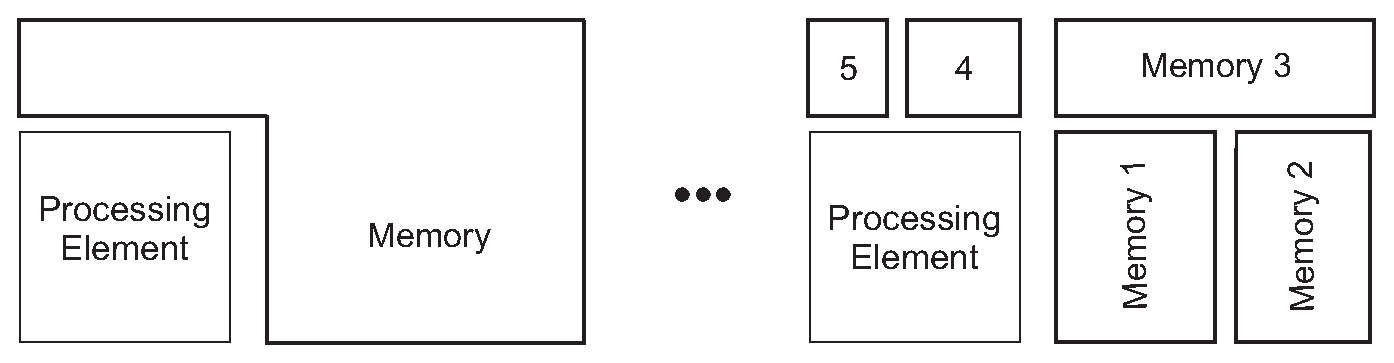
\includegraphics[width=0.45\textwidth]{Images/platform.eps}
\caption{Exploration of memory clustering into varying number of banks}
\label{fig:platform}
\end{figure}

\subsection{Models of different storage types}

\begin{center}
	\begin{table*}[!t]
	\caption{Relative energy for a range of memories with varying capacity and type}
	\label{tab:relative}
	{\small
	\hfill{}
	\begin{tabular}{|c|c|c|c|c|c|c|c|}
		\hline
		\multirow{2}{*}{\textbf{Type}} & \multirow{2}{*}{\textbf{Lines x wordlength}} & \multicolumn{2}{c|}{\textbf{Dynamic Energy}}& \multicolumn{4}{c|}{\textbf{Static Leakage Power per Mode}}\\ \cline{3-8}
		& & Read & Write & Active & Light-sleep & Deep-sleep & Shut-down \\ 
		\hline 
		MM & 32 x 8 &  $ 4.18 \times 10^{-8} $ &  $ 3.24 \times 10^{-8} $ & 0.132 & 0.125 & 0.063 & 0.0016\\ 
		\hline
		MM & 32 x 16 & $  6.79 \times 10^{-8} $ &  $ 5.89 \times 10^{-8} $ & 0.134 & 0.127 & 0.064 & 0.0022\\ 
		\hline
		MM & 32 x 128 & $  4.33 \times 10^{-7} $ &  $ 4.31 \times 10^{-7} $ & 0.171 & 0.160 & 0.083 & 0.0112\\ 
		\hline
		MM & 256 x 128 & $  4.48 \times 10^{-7} $ &  $ 4.60 \times 10^{-7} $ & 0.207 & 0.184 & 0.104 & 0.0293\\ 
		\hline
		MM & 1024 x 128 & $  5.11 \times 10^{-7} $ &  $ 5.75 \times 10^{-7} $ & 0.349 & 0.283 & 0.189 & 0.102\\ 
		\hline
		MM & 4096 x 128 & $  9.60 \times 10^{-7} $ &  $ 4.57 \times 10^{-7} $ & 0.95 & 0.708 & 0.544 & 0.396\\ 
		\hline
		SCMEM & 128 x 128 & $  2.5 \times 10^{-7} $ &  $ 0.8 \times 10^{-8} $ & 0.083 & 0.057 & 0.027 & 0.0022\\ 
		\hline
		SCMEM & 1024 x 8 & $  1.7 \times 10^{-8} $ &  $ 0.6 \times 10^{-8} $ & 0.042 & 0.028 & 0.014 & 0.0011\\ 
		\hline
	\end{tabular}}
	\hfill{}
	\\
	\end{table*}
\end{center}

The dynamic memory organisation is constructed using commercially available SRAM memory models (MM). In addition, experimental standard cell-based memories (SCMEM) \cite{Mei11}  are  considered for smaller memories due to their energy and area efficiency for reasonably small storage capacities, as argued in \cite{Mei10}. Both MMs and SCMEMs can operate under a wide range of supply voltages, thus support different operating modes that provide an important exploration space.

\begin{itemize}
\item Active mode: The normal operation mode, in which the memory can be accessed in the maximum supported speed. The supply voltage is 1.1V and it is expected that the dynamic and leakage power are higher compared to the other modes.
\item Light sleep mode: The supply voltage in this mode is lower than active with values in the area of 0.7V. The access time of the memory in that mode is expected much higher than the access time on active mode. Switching to active mode can be performed with a small time penalty of a few clock cycles, less than 10, and all the data are retained.  
\item Deep sleep mode: The supply voltage is set to the lower possible value that can be achieved without loss of data. This voltage threshold is expected to be lower for SCMEMs than MM models and can be as low as 0.3V. The amount of clock cycles needed for switching to active mode is higher compared to sleep mode. Consequentially, the speed of the PE and the real-time constrains of the applications has to be taken into consideration for deciding, if light or deep sleep mode should be chosen at a specific time.  
\item Shut down mode: Power-gating techniques result to near zero leakage power and retaining of stored data is impossible in this mode. The switch to active mode needs a higher energy and takes more time. However, switching unused memories to this mode, providing that the containing data will not be reused in the future, results to important energy gains.
\end{itemize}  

The necessary energy/power information is available to the system designer and relative values for some of the used sizes in the current work are presented in Tab.~\ref{tab:relative}. It is clearly shown that the choice of the memory units has an important impact on the energy consumption. Moreover, different decisions have to be made based on the dominance of the dynamic or the leakage energy in a specific application. In the current work all memory architectures with up to 5 memory units are explored and the optimal configuration is chosen.

The methodology is in general not restricted to specific memory types or benchmarks and can handle more complex hierarchical memory architectures and applications. However, in this study the chosen applications have a relatively small storage requirement limited to around 100KB, which is the case for many applications run on modern embedded systems. 

\subsection{Energy consumption calculation}

A cycle accurate simulator that supports the described reconfigurable custom memory organisations is not existing and the development of such a simulator is beyond the scope of this work.  Instead the overall energy consumption for each configuration is calculated using a detailed formula, as can be seen in (\ref{eq:energy}). 

\setlength{\arraycolsep}{0.0em}
\begin{eqnarray}
\label{eq:energy}
 E &{}= {}&\sum\limits_{memories}^{all}  ( N_{rd_{acc}} \times E_{Read} \nonumber\\
		&&+ N_{wr_{acc}} \times E_{Write} \nonumber\\
		&&+ (T - T_{Sleep}) \times P_{leak_{Normal}} \nonumber\\
		&&+ T_{Sleep} \times P_{leak_{Sleep}} \nonumber\\ 
		&& + N_{SW} \times E_{SleepNormal}
\end{eqnarray}
\setlength{\arraycolsep}{5pt}

All the important transactions on the platform that contribute to the overall energy are included, in order to achieve as accurate results as possible. In particular:
\begin{itemize}
\item $N_{rd_{acc}}$ is the number of read accesses
\item $E_{Read}$ the energy per read
\item $N_{wr_{acc}}$ is the number of write accesses 
\item $E_{Write}$ the energy per write that is higher in general to the energy per read 
\item T the execution time of the application
\item $T_{Sleep}$ the time spent in sleep state
\item $P_{leak_{Normal}}$ is the leakage power on the active mode 
\item $P_{leak_{Sleep}}$ is the leakage power on the sleep mode with different values corresponding on each sleep mode 
\item $N_{SW}$ the number of transitions from one state to another
\item $E_{SleepNormal}$ the energy for changing states
\end{itemize}

 The overall energy consumption is given after calculating the energy for each memory bank. The execution time of the application is needed for calculating the actual time of leakage, while memory subsystem is on. Execution time and can be given by execution of application's code on a reference embedded processor.   
 
\section{Application Benchmarks}
\label{sec:applications}

\begin{center}
\begin{table*}[!t]
\caption{Benchmark applications overview}
\label{tab:applications}
{\small
\hfill{}
\begin{tabular}{|c|c|c|c|c|}
\hline 
\textbf{Application} & \textbf{Dynamic variable} & \textbf{Memory variation(B)} & \textbf{Source} & \textbf{Characteristics}\\ 
\hline 
Epic image compression & Image size & 4257 - 34609 & MediaBench & Average dynamism, good distribution\\ 
\hline 
Motion Estimation & Image size & 4800 - 52800 & MediaBench & High dynamism, average distribution\\ 
\hline 
Blowfish decoder & Input file size & 256 - 5120 & MiBench & Low dynamism, poor distribution\\ 
\hline 
Jacobi 1D Decomposition & Number of steps & 502 - 32002 & Polybench & Low dynamism, good distribution\\ 
\hline 
Mesa 3D & Loop bound & 5 - 50000 & MediaBench & High dynamism, average distribution\\ 
\hline 
JPEG DCT & Block size & 10239 - 61439 & MediaBench & High dynamism, average distribution\\ 
\hline 
PGP encryption & Encryption length & 3073 - 49153 & MediaBench & High dynamism, average distribution\\ 
\hline 
Viterbi encoder & Constraint length & 5121 - 14337 & Open & low dynamism, good distribution\\ 
\hline 
\end{tabular}}
\hfill{}
\\
\end{table*}
\end{center}

Ideal applications, that can most benefit from memory-aware system scenario methodology, are applications that have dynamic behaviour in memory organisation utilization during their execution. Multimedia applications often exhibit such a dynamic variation on storage requirements during their lifetime and consequentially are suitable candidates for the presented methodology. The effectiveness is demonstrated and tested using a variety of open multimedia benchmarks, which can be found in Polybench (\cite{Poly}), Mibench (\cite{mibench}) and Mediabench(\cite{mediabench}) benchmark suites. Execution of multimedia applications on embedded systems is growing and therefore there is a strong motivation for their study.

\subsection{Presentation of multimedia benchmark applications}

An overview of the benchmark applications that were tested is presented in Tab.~\ref{tab:applications}. Two key parameters under consideration are the dynamic variable on each application and the variation in the storage requirements. The dynamic variable is the variable that results in different scenarios due to its range of values. Examples of such a variable are an input image of varying size or a loop bound with a non-fixed value. The memory size limits are defined as the minimum and maximum storage requirement occurred during testing of application.

\textit{EPIC (Efficient Pyramid Image Coder) image compression} is an algorithm used for compressing an image that can compress all possible sizes of images. The size of the input image has an effect on memory requirements during compression and several images were given as inputs. \textit{Motion estimation} is another media application in which image size is the dynamic variable. In this case the image defines the area that has to be explored for determining the motion vectors and different images are tested.

Dynamism in \textit{blowfish decoder} benchmark is a result of the variations in the input file that is decoded. Again, the methodology explores the behaviour for several input files in order to identify scenarios. \textit{Jacobi 1D decomposition} algorithm can be executed for a varying number of steps with a straight effect on memory usage and so is another suitable benchmark for applying the system scenario methodology. \textit{Mesa 3D} is an open graphics library with a dynamic loop bound in its kernel that provides the desired dynamic behaviour. 

The discrete cosine transformation (DCT) block used on \textit{JPEG compression} algorithm has a memory footprint that is heavily influenced by the block size. The \textit{PGP encryption} algorithm is also included in the employed benchmark suites and its encryption length parameter has an important impact on storage size, that can be exploited using system scenarios. The effect of the SNR level on the channel on the constraint length value on \textit{Viterbi encoder} algorithm is discussed on \cite{Fil12}. The increment of noise in the channel demands a more complex encoding in order to maintain a constant bit error rate (BER), which consequentially increases the memory requirements during algorithms execution. The memory size variation is given for execution under different SNR levels.  

%F: Meta-scenarios
\subsection{Categorisation of applications based on basic characteristics}
\label{sec:categorisation}
The required dynamism for applying the memory-aware system scenario methodology could be produced by several code characteristics, covering a wide range of potential application, as discussed on the previous subsection. Another contribution of this work is the categorization of applications based on their characteristics. It is useful to identify basic characteristics that could lead the system designer towards the employment of the methodology and reveal the expected behaviour prior to experimentation with an application. The basic characteristics that are used to categorize the applications are the dynamism in the storage size bounds and the variance of cases within storage size limits.

The storage bounds correspond to the minimum and maximum memory size values profiled over all possible cases. In general, an increment on distance between upper and lower bounds could increase the possibilities for energy gains. This is a result of using larger and more energy hungry memories in order to support the high storage requirements for the worst case and energy gains are expected in other cases where those memories can be switched into retention for a long time. The group of benchmarks with upper to lower storage size values close to 50KB are JPEG, motion estimator, mesa 3D and PGP. On the other hand, system designer should expect lower energy gains for applications that show a relatively less dynamic behaviour with regard to their storage size limits. Two good examples are blowfish and viterbi algorithms. 

The second metric used for identification of different kinds of dynamism is the variation on memory requirements. The variation takes into consideration both the number of different cases that are present within the storage requirement limits and the distribution of those cases on the space between minimum and maximum memory size. Applications with a limited number of different cases are expected to have much smaller energy gains after a number of platform supported scenarios have been reached. This happens because after a point most of the cases are already optimised for one of the platform configurations and adding new configurations have a minimal impact.

The opposite behaviour is expected for applications that feature a wide range of cases and a good distribution that covers the space between maximum and minimum memory size.

\section{Results}
\label{sec:results}

The memory aware system scenario methodology is applied to all the presented benchmark applications to study its effectiveness. The profiling phase is based on different input for the dynamic variables shown in Tab.~\ref{tab:applications} and is followed by the clustering phase. The clustering is performed starting from one and for up to five scenarios. All potentially energy efficient configurations are tested for a given number of scenarios. The exploration includes memories of different sizes, technologies and varying word lengths. 

The normalized energy consumption is shown in Fig.~\ref{fig:energy} while the energy gain percentages are presented in Fig.~\ref{fig:gains}. Energy gains are compared to a platform configuration with only 1 scenario, which correspond to zero percentage gain in Fig.~\ref{fig:gains}. Only the optimal configuration is presented for each scenario value. The energy is normalized for each application separately. Gains are reported compared to the case of the fixed non-re-configurable platform (1 scenario).

\begin{figure}[!t]
\centering
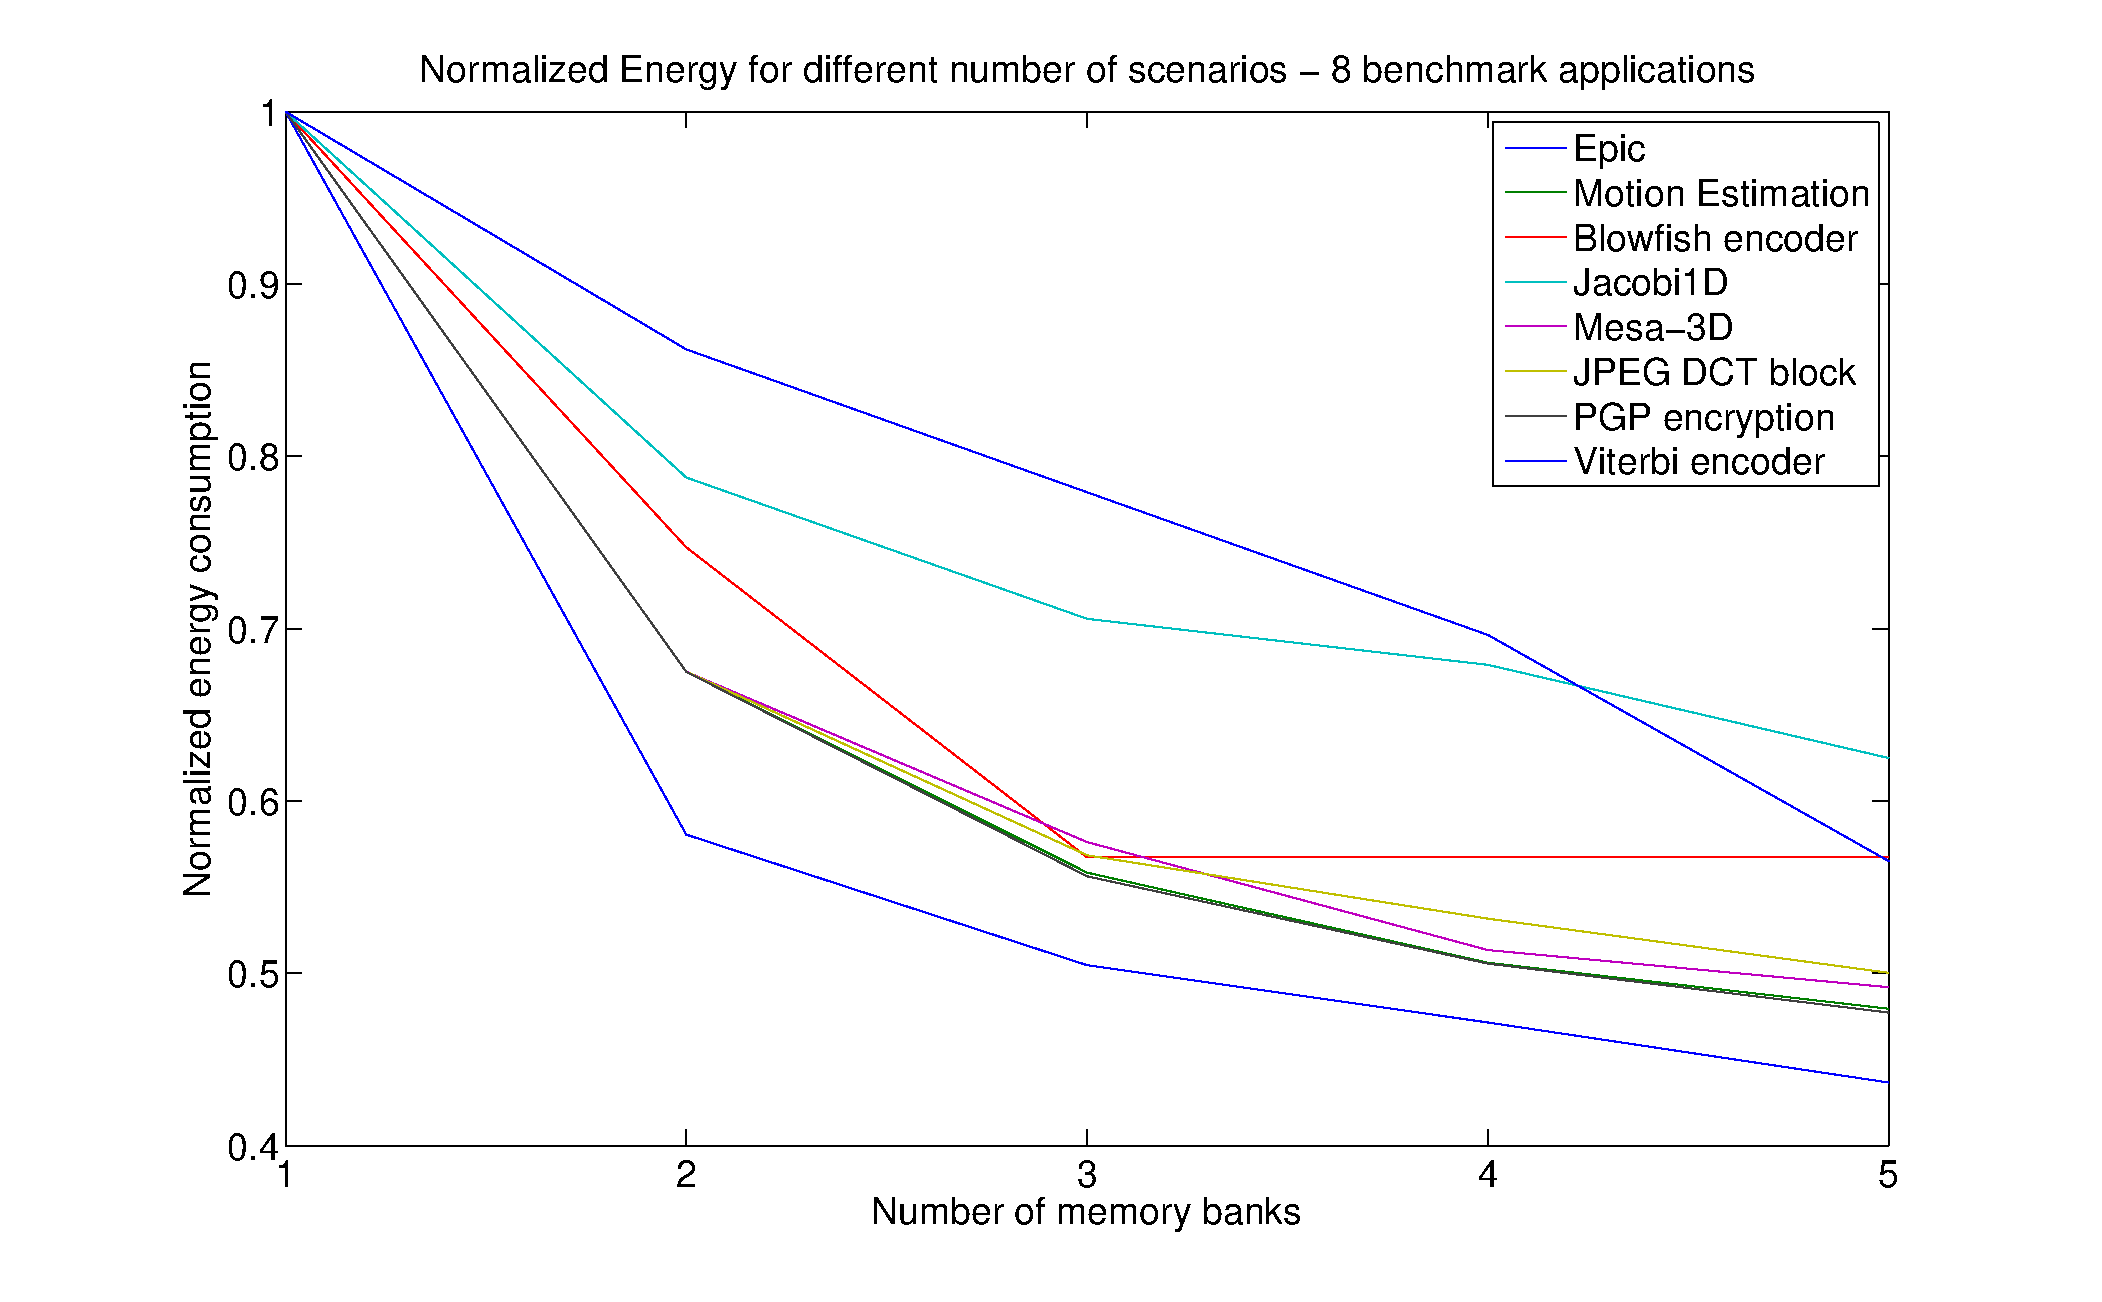
\includegraphics[width=0.45\textwidth]{Images/6apps.eps}
\caption{Energy consumption per number of memory banks - Energy is normalized per application}
\label{fig:energy}
\end{figure}

\begin{figure}[!t]
\centering
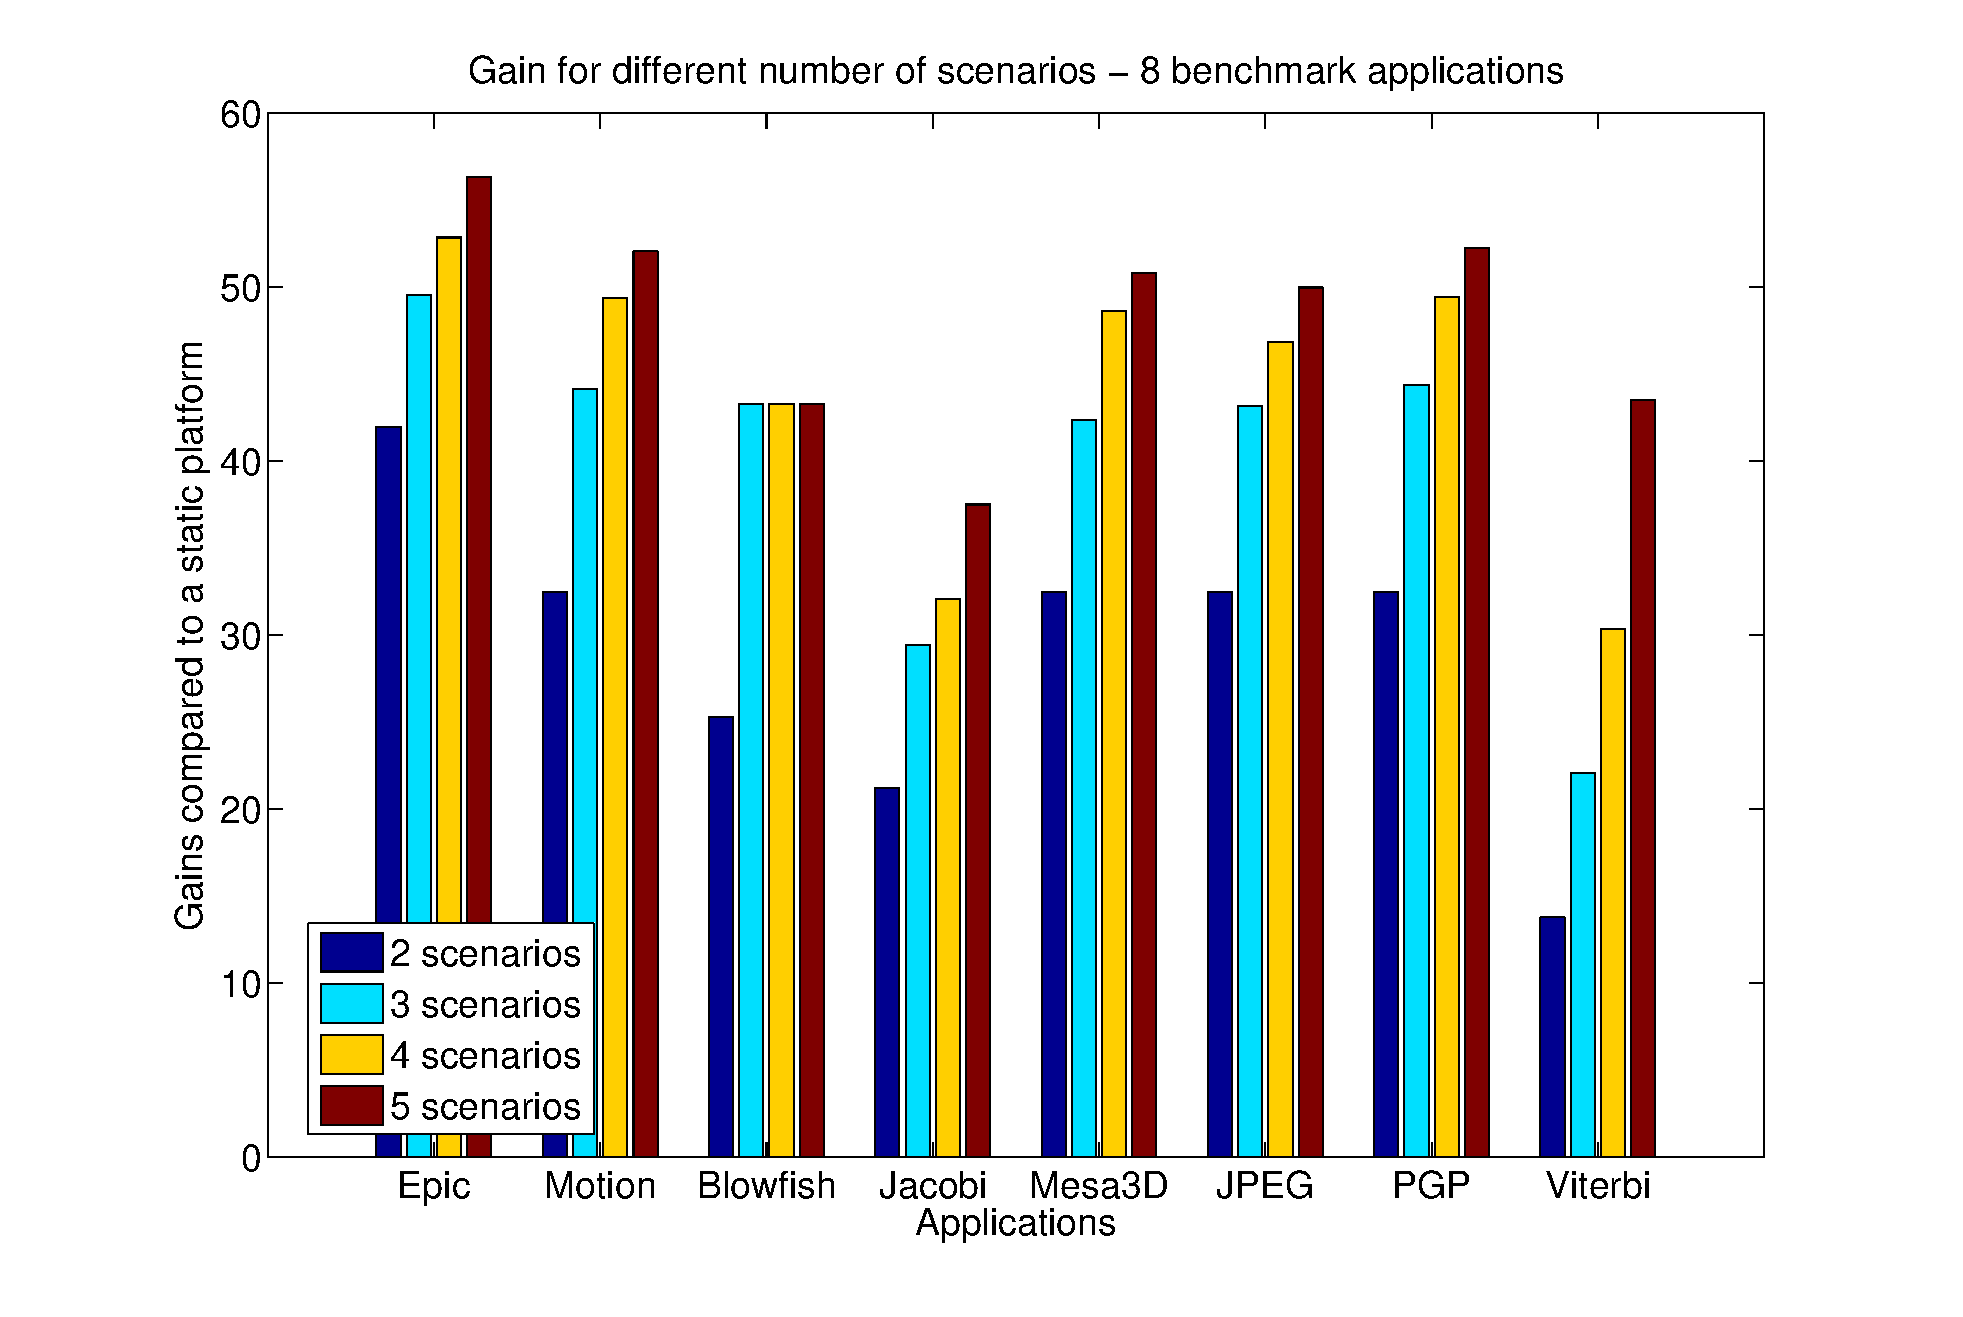
\includegraphics[width=0.48\textwidth]{Images/6appsGains.eps}
\caption{Energy gain for increasing number of scenarios - 1 scenario corresponds to 0\%}
\label{fig:gains}
\end{figure}

The introduction of a second scenario results to energy gains between 15\% and  40\%  for the tested applications. Depending on the application's dynamism the maximum reported energy gains range from around 35\% to 55\%. As expected according to the categorisation presented in subsection~\ref{sec:categorisation}, higher energy gains are achieved for applications with more dynamic storage requirements, i.e. higher difference between the minimum and maximum allocated size, compared to others. The maximum gains for JPEG, motion estimator, mesa 3D and PGP are all above 50\% in contrast to blowfish and Viterbi decoders that are slightly above 40\%.

The increase on the number of scenarios that are implemented on the memory subsystem improves the energy efficient, as variations in storage requirements can be better exploited with more configurations. However, the scaling on energy consumption for an increasing number of scenarios differentiates based on the kind of dynamism present on each application. The application with the higher variation in distribution of memory requirements is the Viterbi encoder/decoder and gains around 10\% for every new memory bank added, even for a platform growing from four to five banks. In contrast, the application with the lowest number of different cases is blowfish and further exploit a platform with more than three banks. Another case in which smaller energy gains are achieved, after a number of platform supported scenarios have been reached, is the PGP. In this benchmark the introduction of more scenarios has an energy impact less than 5\% after the number of three scenarios have reached.

Comparative results using the use case scenario approach as a reference are presented in Fig.~\ref{fig:usecase}. Reported energy gains for both use case scenarios and system scenarios are given assuming a static platform as a base (0\%). Use case scenarios are generated based on a higher abstraction level that is visible as user's behaviour. For example, use case scenarios for image processing applications generate three scenarios, if large, medium and small are the images identified by the user. Accordingly, use case scenarios for JPEG compression identify only low and high compression as options and motion estimation is performed on I,P and B video frames. The scenario identification is more crude compared to identification on the system level and consequentially the reported gains are superior only compared to a static platform or sometimes a platform with only two scenarios.  

\begin{figure}[!t]
\centering
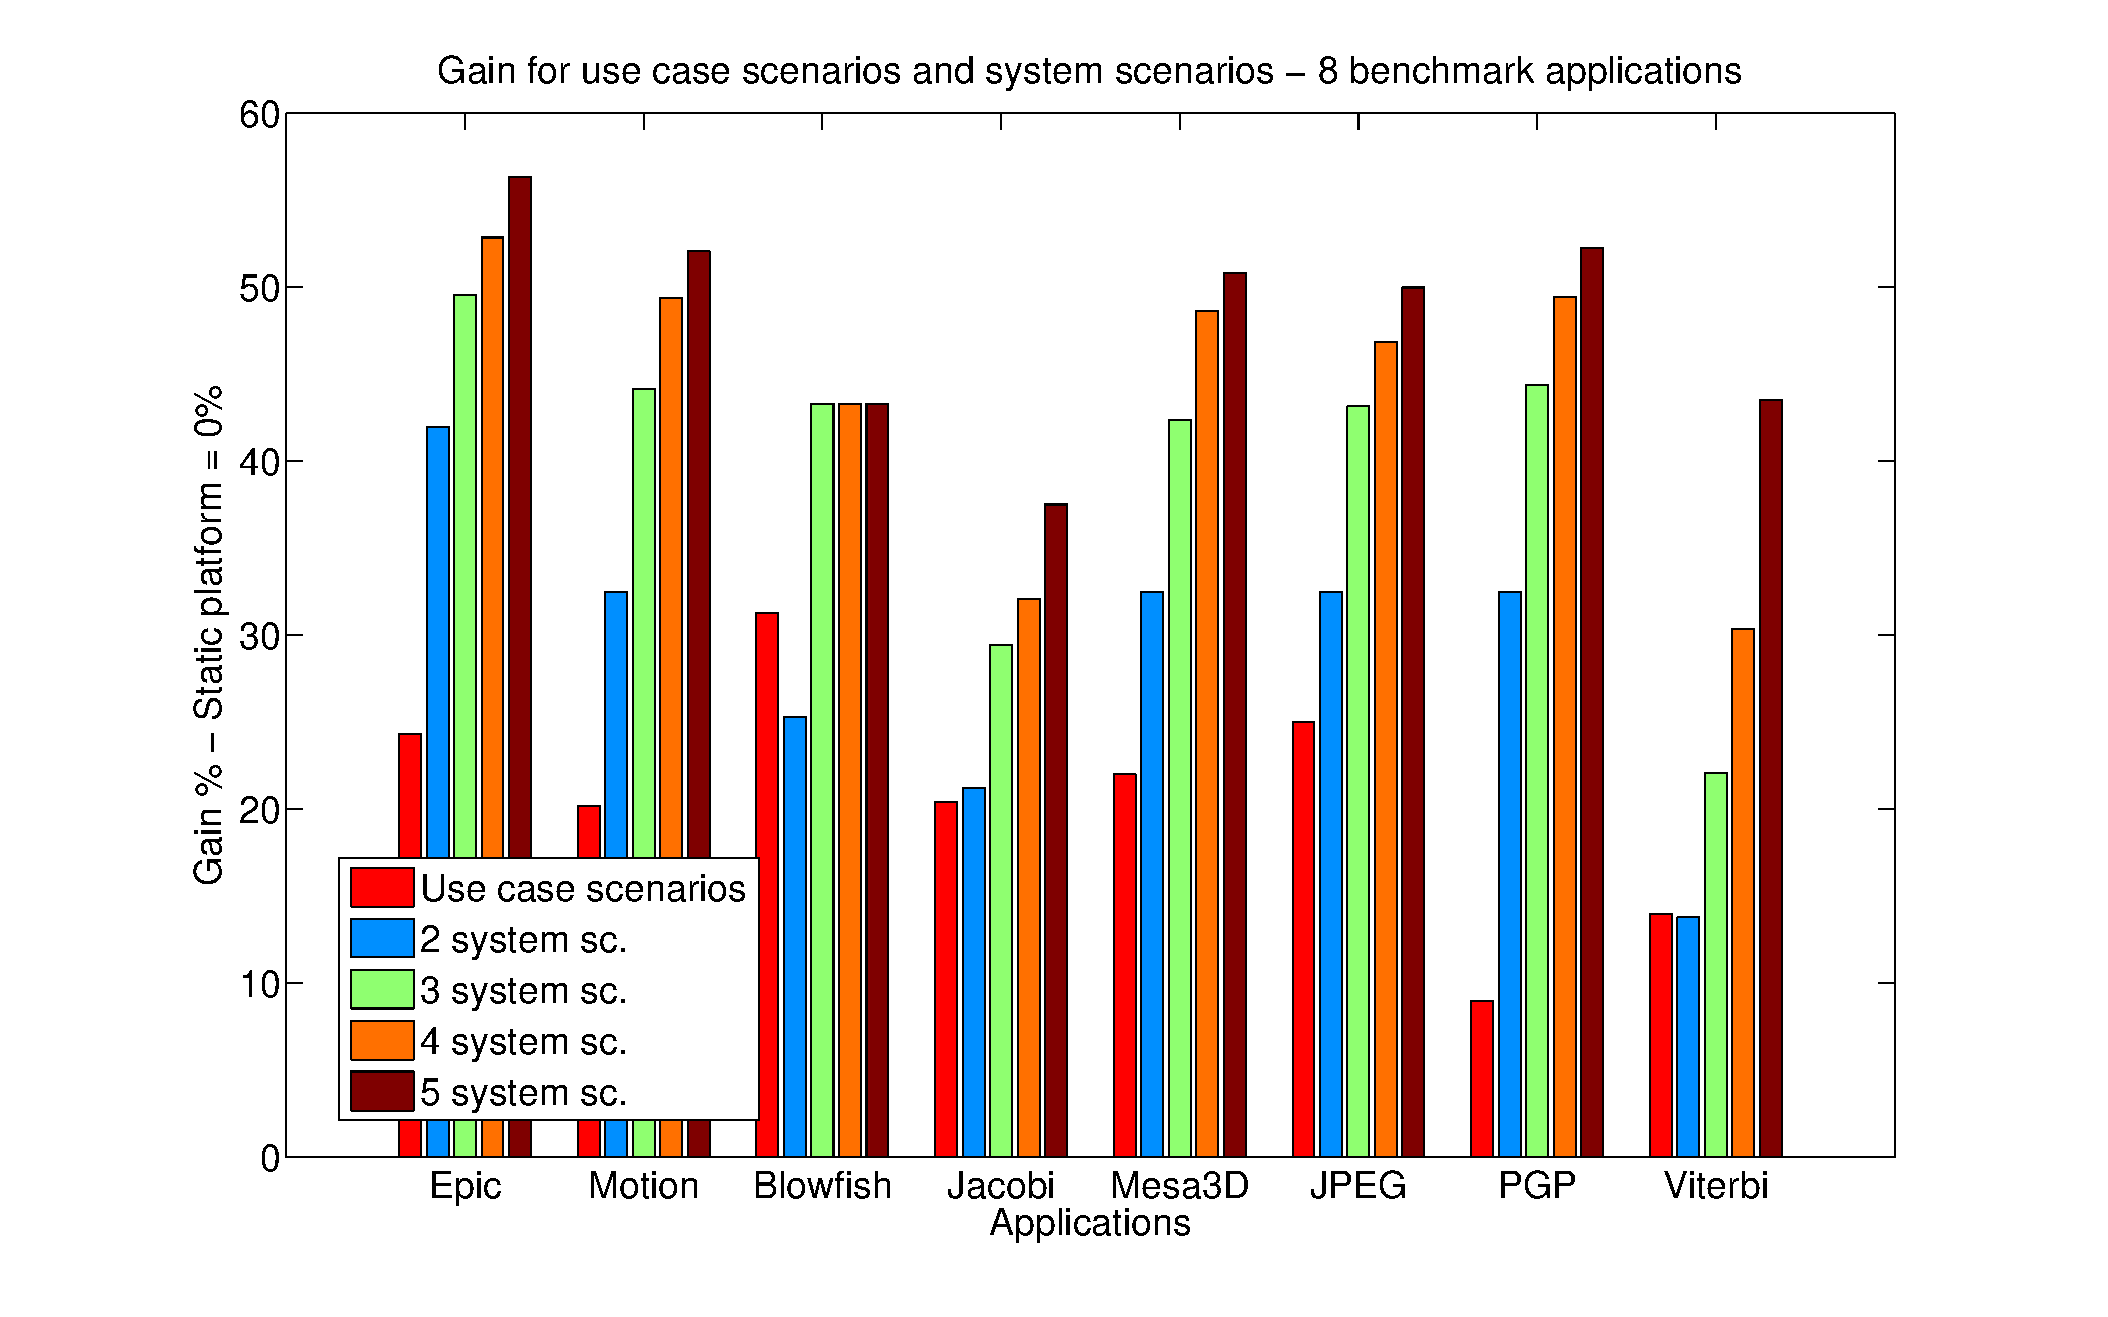
\includegraphics[width=0.48\textwidth]{Images/usecase.eps}
\caption{Energy gain for use case scenarios and system scenarios}
\label{fig:usecase}
\end{figure}

\section{Conclusion}
\label{sec:conclusion}

The scope of this work is to apply the memory-aware system scenario methodology to a wide range of multimedia application and test its effectiveness based on accurate energy models. A wide range of applications is studied that allow us to draw conclusions about different kinds of dynamic behaviour and their effect on application of the methodology. Results justify the effectiveness of the methodology in reduction of memory energy consumption, which is of great importance in embedded devices. Since memory size requirements are still met in all situations, performance is not reduced. The memory-aware system scenario methodology is suited for applications that experience dynamic behaviour with respect to memory organisation utilization during their execution.


\bibliographystyle{IEEEtran}
%\bibliographystyle{plain}
\bibliography{reference}

\end{document}



%CUT

1. Should information about using only MM/SCMEM be included? Report 18
2. 9th and 10th app

from Synopsys\cite{Altera}

The expected behaviour of the benchmark applications can be identified based on some general characteristics